\chapter{Utilizzare le coordinate}

{ }\hfill\textbf{Livello:} Principiante
\section{Presentazione}
In questo capitolo scopriremo la primitiva \texttt{ImpostaPosizione, ImpPos}. L'area di disegno ha due assi che permettono di determinare ciascun punto utilizzando il sistema di coordinate cartesiano. L'origine degli assi è il centro dell'area di disegno.\\
Il formato della primitiva è \texttt{ImpostaPosizione elenco} come in \textcolor{red}{ \texttt{ImpPos [100 -250]}}. La tartaruga si sposta al punto di coordinate X 100 e Y -250. Le coordinate sono racchiuse in parentesi quadre perché la primitiva richiede un elenco. Ricorda che la tartaruga ha una penna che può toccare l'area di disegno o essere alzata. Quando la penna è abbassata la tartaruga disegnerà una linea ogni volta che se ne imposterà la posizione.\\
Un piccolo esempio: \lstinline!PulisciSchermo ImpPos [200 100] ImpPos [50 -150] ImpPos [-100 -150]!.
\begin{center}
	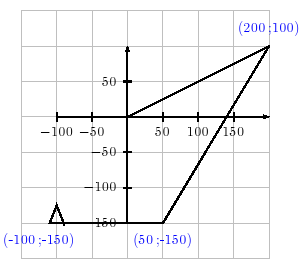
\includegraphics[scale=0.7]{pics/fpos-coord.png}
\end{center}
\vfill


\section{Esercizio}
Prova a disegnare questa figura usando solo le seguenti primitive: \texttt{ImpPos}, \texttt{PScÅ}, \texttt{PS}, \texttt{PG}.\\
\begin{center}
	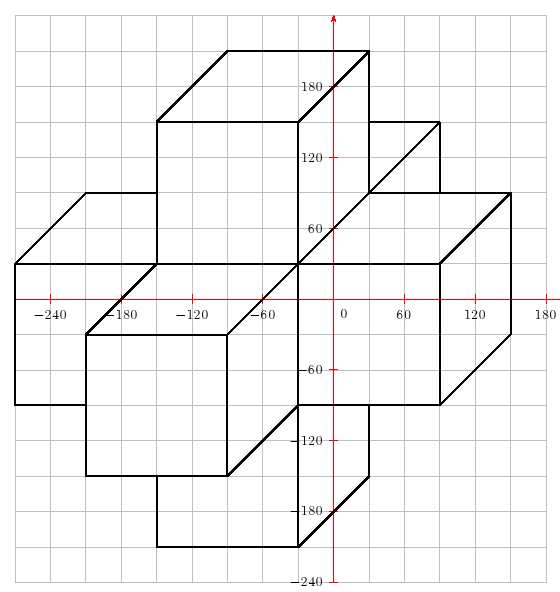
\includegraphics[scale=0.7]{pics/fpos-cube.png}
\end{center}